\documentclass[12]{article}
%\usepackage[utf8]{inputenc}
\usepackage{lmodern,textcomp}
\usepackage{hyperref}
\usepackage{graphicx}
\usepackage{float}
\usepackage[spanish]{babel}
%\usepackage{listings}


\title{Red Anónima I2P}
\author{Borja Fernández Merchán \\ Andrés Gomar Pérez \\ Carlos Rodrigo Sanabria Flores \\ Sergio Ruiz Pino
 \\ Iván Piña Arévalo}
\date{\today}

\begin{document}
\maketitle

\section{Introducción}
En este trabajo realizaremos un estudio sobre la tecnología I2P. En el presente Internet forma parte de la vida 
de millones de personas y afortunadamente cada vez somos más conscientes de la importancia de los datos. El bien 
más preciado para muchas empresas es precisamente los datos de sus potenciales clientes. Además, con casos tan 
flagrantes como Cambridge Analytics o las fugas de información a las que desafortunadamente estamos acostumbrados. 

Tal vez un sentimiento similar surgió en la persona que se esconde bajo el pseudónimo ‘jrandom’. Bajo este 
pseudónimo se oculta la mente que esta al cargo del proyecto I2P. Pero antes pongamos un ejemplo que puede resultar 
esclarecedor para entender.

Supongamos a un activista, dicho activista está en contra de las medidas que se están tomando en su país contra 
la fauna y flora que habita allí. Sin embargo, debido a las relaciones diplomáticas con los países de su alrededor
y a la represión mediática, dicha información no traspasa las fronteras nacionales, impidiendo que se sepan las desastrosas 
decisiones que se están llevando a cabo. En este caso lo más importante para el activista no es la información en si misma 
ya que la conocen centenares o miles de personas. Lo más importante es que no se conozca su verdadera identidad ya que 
automáticamente seria localizado y según la normativa del país podría incluso ser ejecutado. 

En respuesta a este tipo de situaciones surge el concepto de redes anónimas. En este tipo de redes el objetivo principal es 
el anonimato. El objetivo principal de Internet cuando surgió fue la transmisión de información, no la privacidad de esta. La 
capa que subyace a este tipo de tecnologías es el enrutamiento basado en capas de cebolla. De esta manera conseguimos que cada 
nodo conozca únicamente su nodo anterior y siguiente en lugar de los nodos origen y final. Otro aspecto fundamental para conseguir 
la deseada privacidad consiste en el desacomplamiento del emisor y su mensaje. De esta forma conseguimos ganar anonimato en las 
transmisiones. 

Cabe destacar una particularidad de la red I2P. Se puede observar como si fuera una intranet. Esta característica en si misma se podría ver 
como una mejora de seguridad ya que limitamos el número de tecnologías y dispositos capaces de acceder desde el exterior. Al limitar las tecnologías 
empleadas reducimos el número de posibles amenazas, en otras palabras, podemos prestar más atención a la tipología de los ataques. 

Por los motivos mencionados anteriormente y el momento actual en el que vivimos, realizar un estudio acerca de una tecnología que 
pone su enfoque en la privacidad del usuario resulta esperanzador. Por supuesto es un arma de doble filo ya que puede ser empleada con fines 
perversos, pero no deja de ser una herramienta, todo depende del uso que queramos hacer de ella.

\pagebreak

\section{Descripción de la tecnología I2P}

I2P (\textit{Invisible Internet Project}) es lo que se conoce como una capa de red anónima P2P. Esto es, una red \textbf{descentralizada}, basada en el empleo de múltiples nodos anónimos interconectados
que hacen posible la comunicación entre dos usuarios; cabe destacar la palabra "capa", pues I2P es lo que se conoce como un \textit{overlay network}, una red funcionando encima de otra red. Es un concepto
de capas con mucha similitud a la estructura de una cebolla, como veremos más adelante.

El principal objetivo del proyecto es proteger el anonimato de los usuarios de la red; para esto, I2P implementa una \textit{red mix}.

\subsection{Redes Mix}
El concepto de las redes mix existe desde 1981 [7] se utilizan una serie de servidores \textit{proxy} intermedios llamados \textit{mix} que proporcionan múltiples
capas de seguridad a la comunicación. De forma breve, el papel de los \textit{mix} consiste en recibir un mensaje, que viene cifrado especialmente para ellos,
y enviarlo al siguiente destinatario (probablemente otro \textit{mix}).
El sistema funciona y otorga anonimato por hacer irrastreable al emisor original, ya que cada \textit{mix} solo tiene información del siguiente punto de envío, de forma que ninguno de ellos conoce
ni el mensaje, ni la procedencia, ni la ruta completa.

\begin{figure}
    \centering
    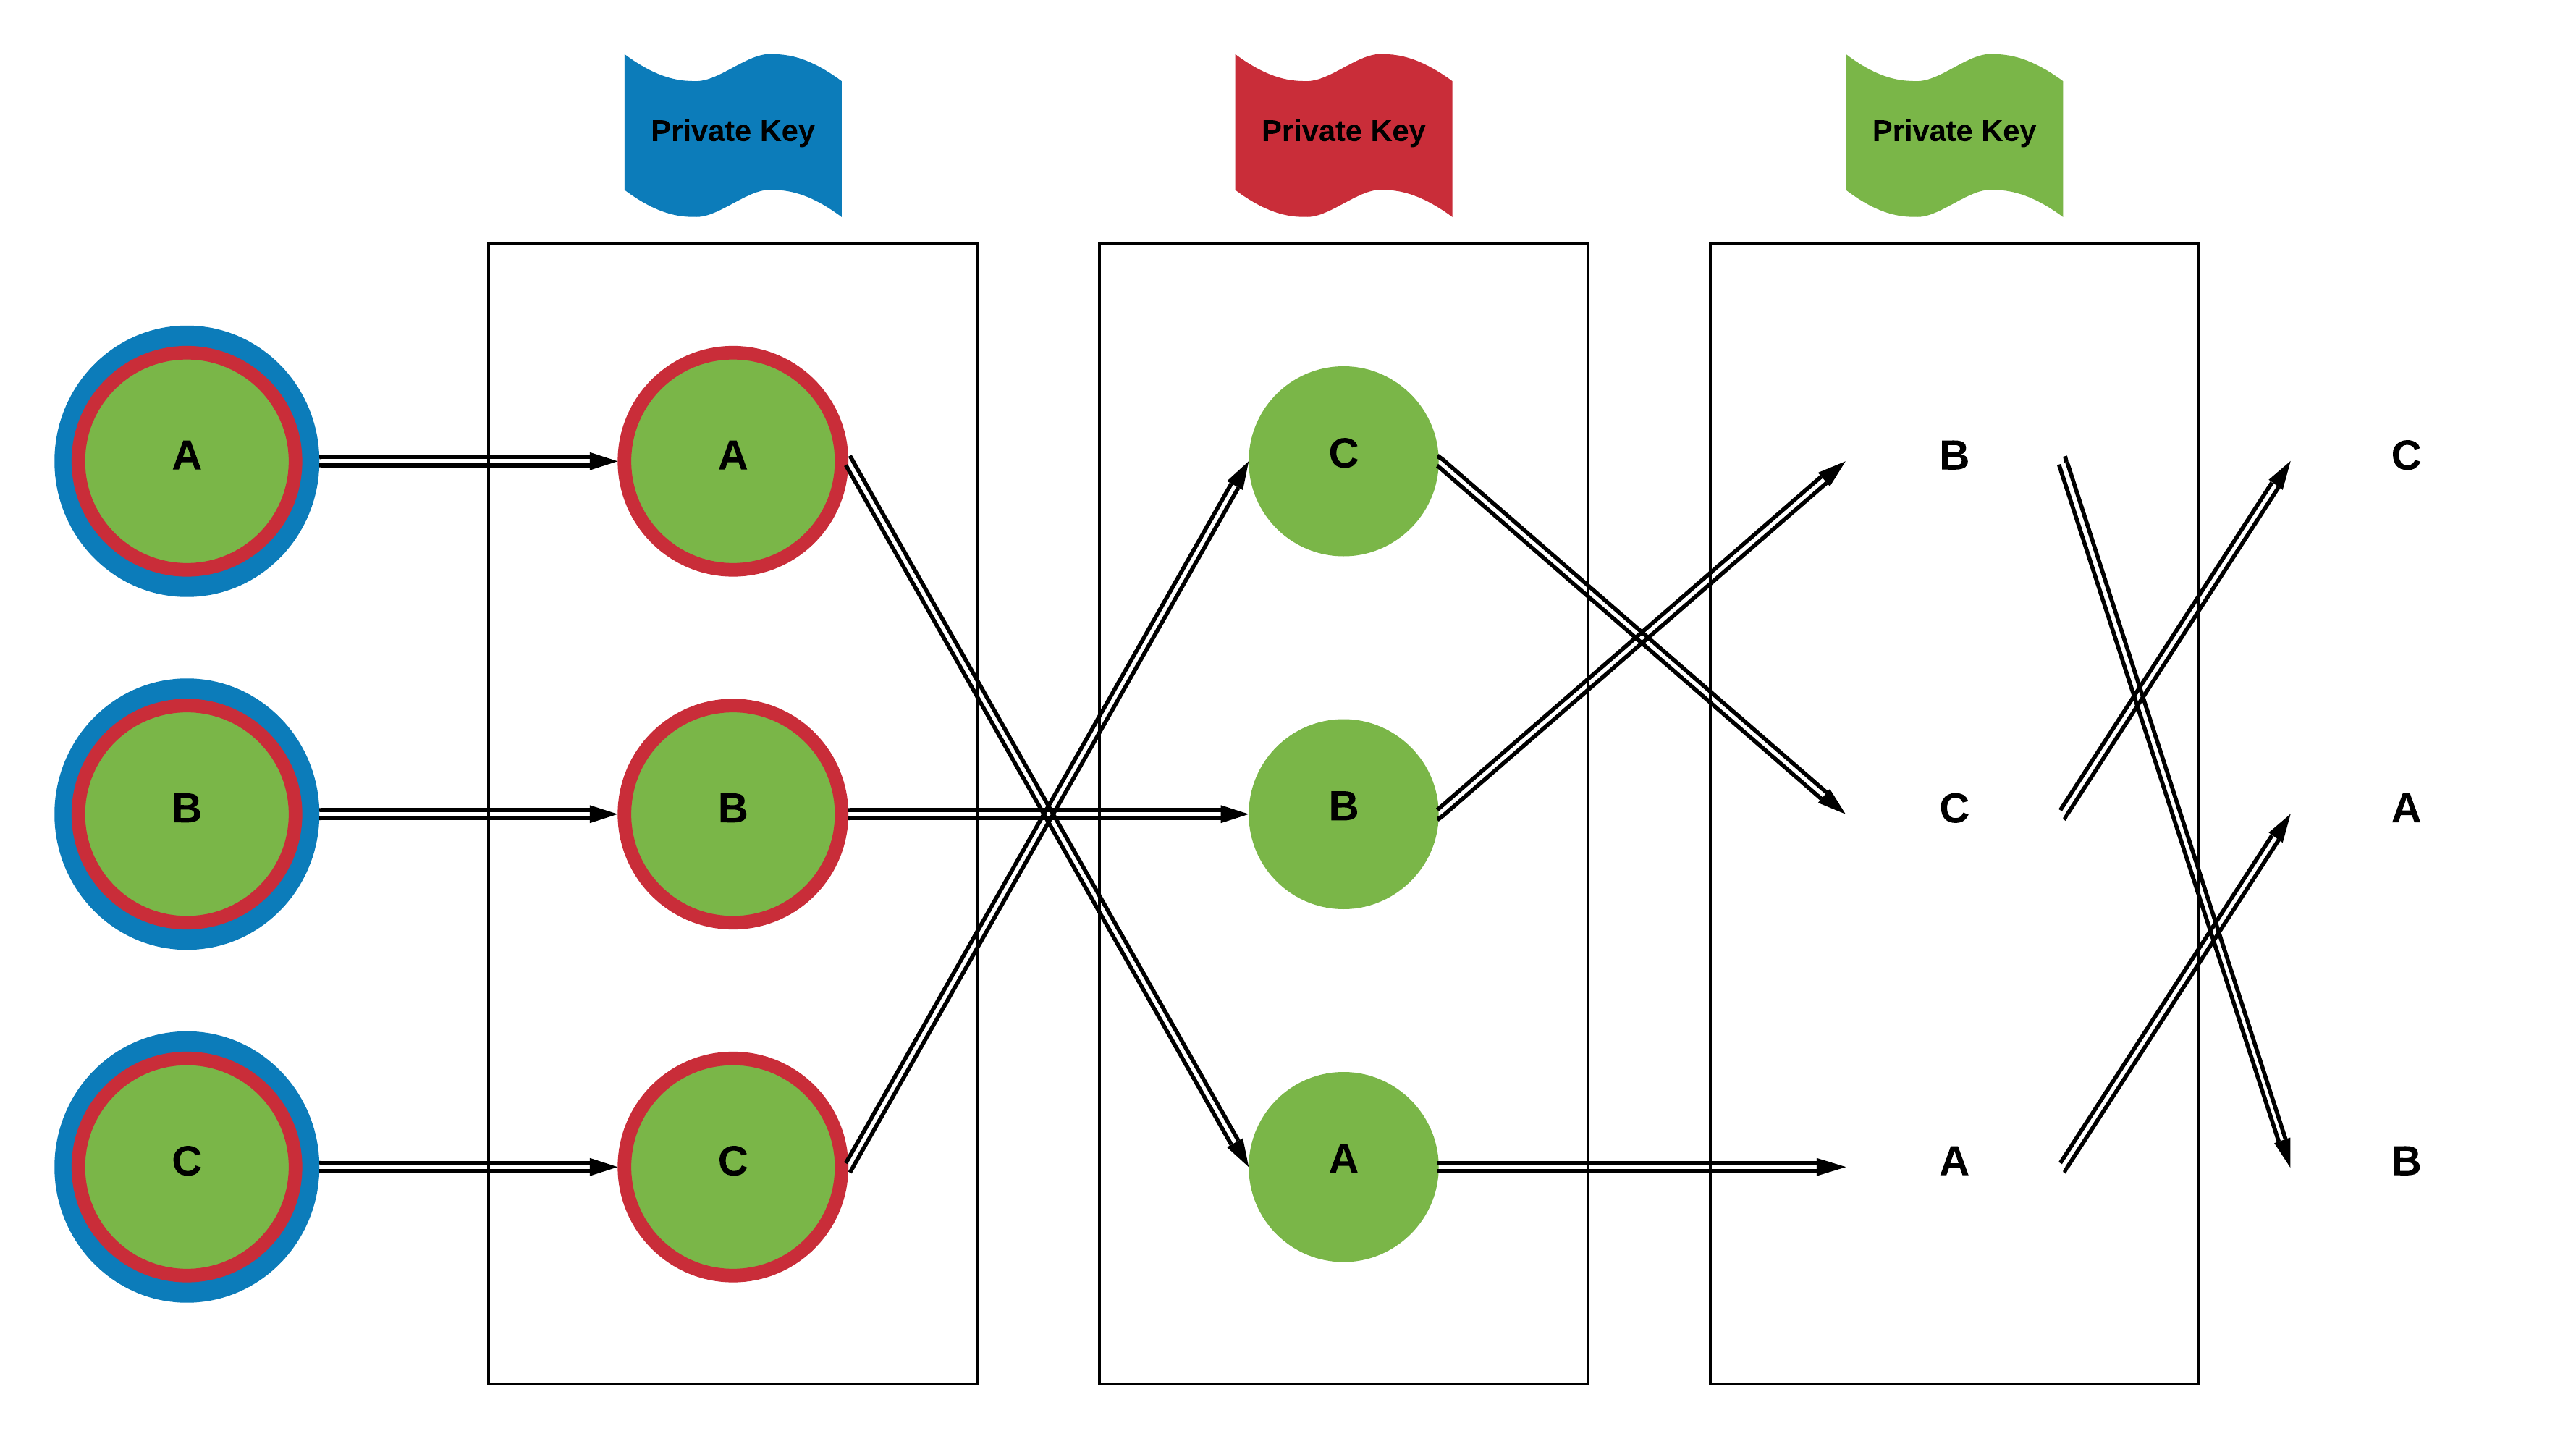
\includegraphics[width=\linewidth]{media/Mix Network.png}
    \caption{Funcionamiento de una red Mix.}
    \label{fig1}
\end{figure}

Las redes \textit{mix} se basan en paso de mensajes, por lo que toda la protección que implementan orbitan en torno a ellos. Los mensajes en una red \textit{mix} son como
muñecas \textit{Matryoshka} \footnote{las muñecas Matryoshka son unos populares juguetes de origen ruso que consisten en un set de piezas huecas, de forma ahovada y diferentes tamaños,
pintadas por fuera para parecer mujeres. Al tener diferentes tamaños, se pueden ir guardando unas dentro de otras, hasta que finalmente todas las piezas del set están dentro de la pieza mayor.}
con la excepción de que todas las piezas son iguales en forma (y, por tanto, tamaño) si descontamos el mensaje interno que llevan (lo que sería la siguiente capa).

Pongamos un ejemplo para entender mejor las redes \textit{mix}. Un emisor, \(A\), quiere enviar un mensaje a un receptor, \(B\). Para asegurarse de que solo B lea el mensaje, A debe encriptarlo
con la clave pública de B, \(K_b\). Sin embargo, si un tercero, \(C\) interceptase el mensaje, y también tuviese la clave pública de B, podría llegar a averiguar el contenido del mensaje \footnote{al ser el algoritmo
de encriptación determinista, para una misma entrada (mensaje y clave pública) el atacante tan solo tendría que probar mensajes hasta que obtuviera el mismo resultado cifrado que el interceptado, conociendo
de esta forma el contenido del mensaje.}. Para evitar esto, al encriptar el mensaje, A añadirá una cadena aleatoria, \(R_0\), que funcionará esencialmente como \textit{sal}\footnote{el concepto de "sal"
responde a un argumento adicional, como en el caso del mensaje encriptado, que impide romper la encriptación de un algoritmo determinista al añadir un tercer valor, desconocido, aleatorio, y normalmente tan
largo, que imposibilita obtener el mensaje sin conocer la clave para descifrarlo} de la encriptación. De esta forma, el mensaje que A quiere enviar a B, queda así: \[K_b (R_0, mensaje)\].

Ahora, A debe enviar el mensaje a un \textit{mix}. La confidencialidad de B es primordial también, por lo que su dirección (junto con el mensaje encriptado) se encripta con la clave pública del \textit{mix},
\(K_m\). De nuevo, acorde a lo que hemos explicado, añadimos una sal aleatoria al encriptado, \(R_1\), de forma que el mensaje que manda A al \textit{mix} es el siguiente: \[K_m(R_1, K_b(R_0, mensaje), B)\]

Dependiendo del número de \textit{mix} que vaya a recorrer el mensaje, tantas capas adicionales tendrá. Dado que cada capa solo puede ser desbloqueada por un \textit{mix} concreto, interceptar
el mensaje carece de utilidad alguna para el hipotético atacante, C. Para añadir saltos adicionales, basta con repetir el procedimiento que hemos explicado: se añade una sal aleatoria, y la dirección
del siguiente \textit{mix} en la cadena, y luego se encripta con la clave pública del mismo. De esta forma, si A quisiese enviar su mensaje primero por \textit{mix} 1, y luego por \textit{mix} 2,
el resultado sería el siguiente: \[K_m(R_2, K_b(R_1, K_b(R_0, mensaje), B), M_2)\]

\subsection{Implementación de I2P}

La red I2P implementa este sistema de redes \textit{mix} por medio de voluntarios que ofrecen sus ordenadores para actuar como nodos. Cualquier ordenador puede convertirse en un nodo de la red
I2P simplemente instalando el software "I2P router" [8], que puede consumir tan poco como 128MB de memoria RAM, pudiendo correr incluso en una modesta Raspberry Pi [9].
Dado que cada nodo conoce tan solo la dirección del siguiente nodo (o del destinatario de un mensaje, en caso del último nodo), rastrear una conexión es prácticamente imposible, y puesto que el camino
hacia el destinatario está también encriptado, y cada paso del mismo es conocido solo por cada nodo, interceptar el mensaje al principio tampoco aporta información sobre el mismo.

\begin{figure}[H]
    \centering
    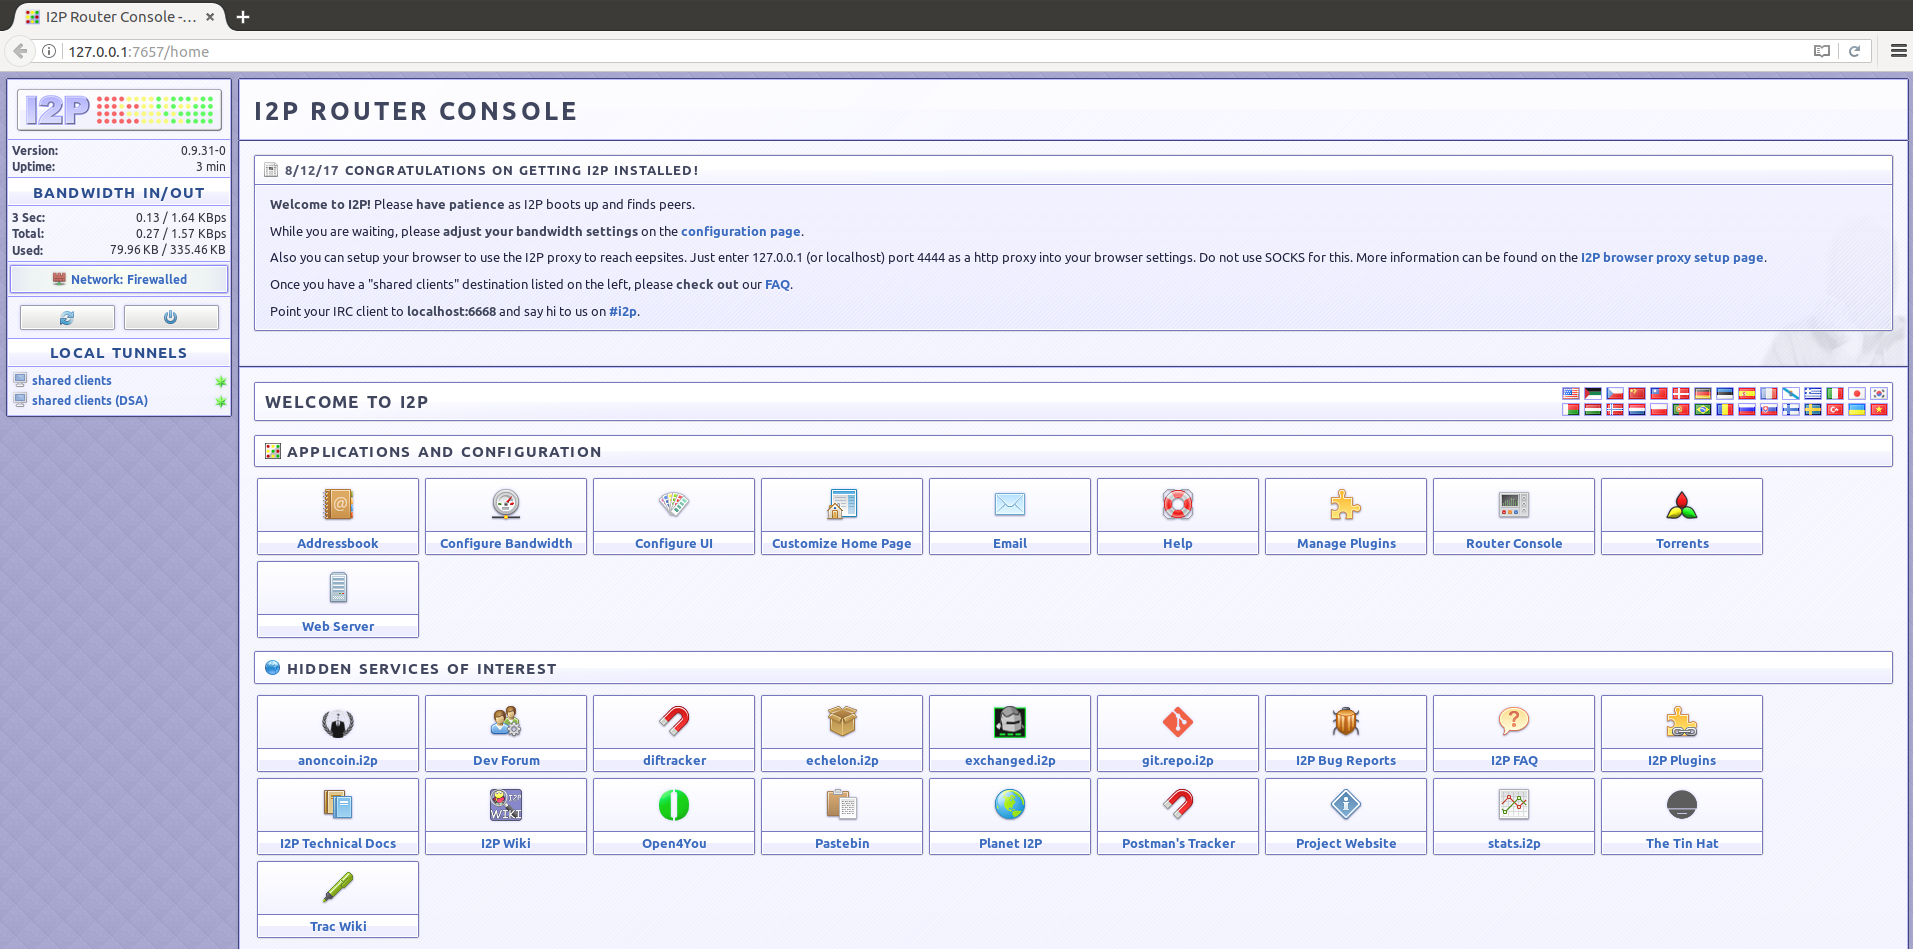
\includegraphics[width=\linewidth]{media/I2P Router Console.png}
    \caption{Captura de la consola del router I2P.}
    \label{fig2}
\end{figure}

Para añadir seguridad adicional al sistema de redes \textit{mix}, la red I2P implementa una versión mejorada del concepto de "\textit{onion routing}" llamado, de forma socarrona, "\textit{garlic routing}",
haciendo referencia a su modo de funcionamiento, mediante el cual se empaquetan varios mensajes dirigidos a un mismo destinatario (de ahí el simil con los dientes de ajo),
de forma que se hace imposible, incluso si se atrapa el "ajo" al completo, averiguar el contenido de cada mensaje individual.[10]
Dado que el sistema se basa estrictamente en el sistema de paso de mensajes (como las comunicaciones IP), han añadido librerías que emulan el funcionamiento de otros protocolos más complejos,
que permiten llevar a cabo labores de \textit{streaming} (de forma parecida a TCP).

En la actualidad, el proyecto I2P ofrece clientes para multitud de sistemas operativos: Windows, Mac OSX, Debian/Ubuntu, Solaris, GNU/Linux, Android, y BSD; dado que todo el software
(al ser una capa de abstracción que corre por encima de las redes normales) es ejecutado sobre una máquina virtual de Java (\textit{JRE 7+}) goza de una fácil portabilidad.

\begin{figure}[H]
    \centering
    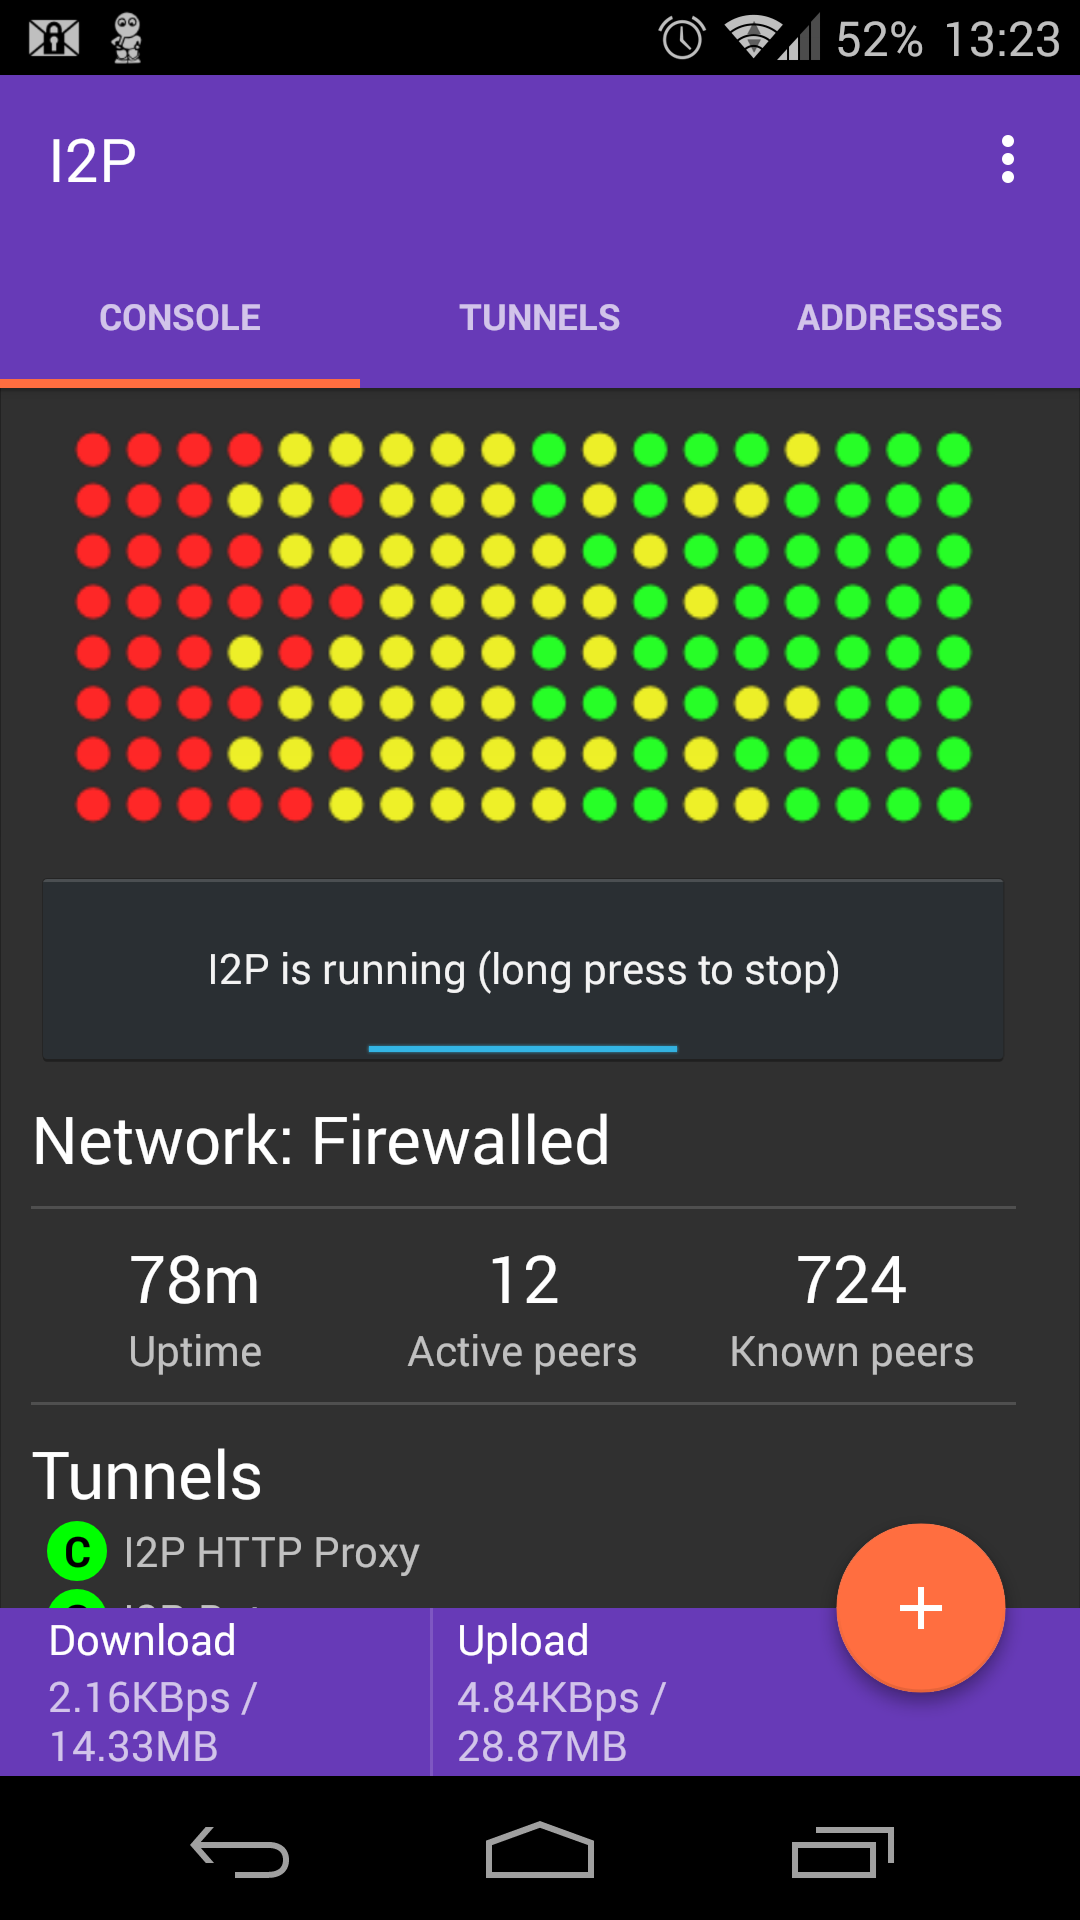
\includegraphics[width=1\textwidth]{media/I2P Android Console.png}
    \caption{Captura del cliente de Android I2P.}
    \label{fig3}
\end{figure}


\section{Casos de estudio en el que se aplica la plataforma/tecnologia I2P}

En el caso de la web, el ideal no cambia, es decir, lo que se busca es usar comunicaciones cifradas para mantener la privacidad de las páginas que visitan los usuarios mediante saltos entre los nodos de la red. A continuación se muestra un ejemplo de como se produce el salto entre nodos.

\begin{figure}[H]
    \centering
    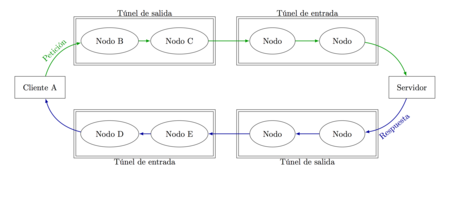
\includegraphics[width=1\textwidth]{media/salto_nodos.png}
    \caption{Salto entre nodos I2P.}
    \label{fig4}
\end{figure}

Hay que destacar que en cuanto a las diferentes tecnologías actuales, si lo que queremos es conectarnos a internet a modo de proxy,  Tor es más eficiente que I2P, desventaja de ésta última que la hace más privada que las demás tecnologías al tener menos usuarios siendo mas resistente a ataques hacia la privacidad.[1]

Hay actualmente diversos estudios de investigación referente a la confiabilidad y seguridad de las comunicaciones que se producen en el día a día.
Existe una gran preocupación que concierne a los programas de vigilancia en la web aplicados en plataformas como Facebook, amazon, Google … Esto ha llevado a un colectivo a realización investigaciones para ver de que manera se puede proteger la integridad de los datos. El objetivo de estas investigaciones a llevado a obtener soluciones que nos permitan transferir datos sin que haya terceros
en la red que puedan interceptar éstos.
Una solución propuesta es usar tecnología I2P para asegurar las comunicaciones en la red. Enviamos paquetes desde uno de los túneles de salida hacia un túnel de entrada  impidiendo que nadie puede interceptarlos salvo el receptor del paquete.[2]

Un ejemplo de implementación de I2P es el aseguramiento de privacidad en las comunicaciones sobre internet.
La aparición de nuevas tecnologías ha conllevado la preocupación de colectivos centrados en la privacidad de los datos que se tratan en la red en un ámbito público o privado.

El proyecto I2P se encuentra en auge y continua evolución para garantizarnos el 100 por ciento de seguridad e integridad de los datos y paquetes que se manejan en la red. Éste se  es resistente a ataques masivos posibilitando la ejecución de varias aplicaciones a 
la vez ya que consta de varios modelos a nivel de seguridad y rendimiento para cada usuario que aplican esta tecnología. Las aplicaciones que se basan en esta tecnología se usan básicamente en internet, en la sección de navegación web anonimo por ejemplo.[3]

\subsection{Script para transformar direcciones de i2p en una mas pequeña}

 El siguiente script transforma direcciones de base64 de 500 caracteres a b32.i2p :
 
 \#!/usr/bin/env python3
import base64, hashlib, sys

if len(sys.argv) != 2:
  print('Usage: convertkey.py <base64key>')
  sys.exit(1)

key = sys.argv[1]
raw\_key = base64.b64decode(key, '-~')
hash = hashlib.sha256(raw\_key)
base32\_hash = base64.b32encode(hash.digest())
print(base32\_hash.lower().decode("utf-8").replace("=", "") + ".b32.i2p")
 
/subsection{¿Qué es una "eepsite"?}
Un eepsite es un sitio web alojado de forma anónima, un servicio oculto al que se puede acceder a través de su navegador web. Se puede acceder configurando el proxy HTTP de su navegador web para usar el proxy web I2P (normalmente escucha en el puerto local 4444) y navegando por el sitio.

Es fácil configurar eepsites, pero no se puede conocer fácilmente la dirección IP real de eepsites. Por ejemplo, estoy ejecutando un sitio web llamado legwork.i2p (un motor de búsqueda en la red I2P), se puede acceder fácilmente, pero es posible que no pueda conocer la red o la ubicación física del servidor donde se hospeda. Los sitios web equivalen aproximadamente a los servicios ocultos de Tor.

\pagebreak

\section{Trabajos relacionados de la plataforma/tecnología I2P}

Al ser  I2P una capa de abstracción para asegurar comunicaciones anónimas,existen software que hacen uso de esto.
\\

Destacamos que la existencia de los siguientes software tiene como objetivo preservar nuestro anonimato en la red,y que el objetivo de estos no es solo preservar
el anonimato, sino que sean compatible con otros protocolos de red, así podemos usar aplicaciones en red,que de otra forma, seriamos rastreables,
a continuación explicaremos tres software,que consideramos que su en I2P  es indispensable.
\subsection{I2PTunnel[4]}

Es una herramienta que permite la comunicación sobre I2P, a aplicaciones TCP/IP,su funcionalidad se basa en la creación de tuneles que pueden ser accedidos
conectandonos a puertos.Esta aplicación existe para poder comunicarnos con aplicaciones que usen TCP/IP de forma anonima , es una ventaja ya que si usaramos la aplicación TCP/IP de forma 'normal'
nuestro anonimato no estaría asegurado,
\\

Para configurar I2PTunnel debemos modificar el fichero tunnels.conf,este archivo utiliza el formato de archivo .ini y está diseñado para soportar múltiples túneles I2P. El archivo 
de configuración debe ubicarse en  ~/.i2pd (por usuario) o /var/lib/i2pd (en todo el sistema),podemos configurar tuneles http, udp, servidor y cliente.Los tuneles tienen los 
siguientes parametros.
\\


\subsubsection{Opciones de configuración de tunnels.conf[11]}
inbound.length: número de saltos de un túnel entrante. 3 por defecto; menor valor es más rápido pero peligroso
\\

outbound.length: número de saltos de un túnel de salida. 3 por defecto; menor valor es más rápido pero peligroso
\\

inbound.quantity: número de túneles de entrada. 5 por defecto
\\

outbound.quantity: número de túneles de salida. 5 por defecto
\\

crypto.tagsToSend: número de etiquetas ElGamal / AES para enviar. 40 por defecto; un valor demasiado bajo puede causar problemas con la construcción del túnel
\\

explicitPeers: lista de direcciones b64 separadas por comas de pares para usar, valor predeterminado: sin establecer
\\

i2p.streaming.initialAckDelay: milisegundos a esperar antes de enviar Ack. 200 por defecto
\\

i2cp.leaseSetType: tipo de LeaseSet que se enviará. 1, 3 o 5. 1 por defecto
\\

i2cp.leaseSetEncType: tipo de cifrado que se utilizará en LeaseSet tipo 3. Tipo de identidad por defecto
\\

i2cp.leaseSetPrivKey: clave de descifrado para LeaseSet cifrado en base64. PSK o DH privado
\\

i2cp.leaseSetAuthType: tipo de autenticación para LeaseSet cifrado. 0: sin autenticación (predeterminado), 1: DH, 2: PSK
\\

i2cp.leaseSetClient.dh.nnn - nombre del cliente: DH público del cliente en base64, para el tipo de autenticación 1, nnn es entero
\\

i2cp.leaseSetClient.psk.nnn - nombre del cliente: PSK del cliente en base64, para el tipo de autenticación 2, nnn es entero 
\subsection{I2PSnark[5]}
Permite conectarnos a redes p2p de forma totalmente anonima,ya que si no usamos I2P, y nos conectamos a una red p2p, seriamos rastreables.
\\

Su funcionamiento es similar a un cliente de torrent,agregamos torrent y estos se descargan conectandonos a la red p2p donde se localizen los archivos a descargar,a continuación 
una guia para proceder a su instalación y uso:
\\

1) Descargue el instalador I2P para Windows o Linux
\\

2) Instale la aplicación. Simplemente ejecute el ejecutable en Windows o instale desde terminal en linux.
\\

3) Vaya al menú de inicio y abra la carpeta I2P allí. Haga clic en init I2P.
\\

4) Tiene que configurar un proxy local. Lo hara de la siguiente manera según su navegador:
\\

4.1) Firefox: vaya a Herramientas> Opciones. Haga clic en Avanzado> Red y seleccione el botón Configuración de Conexión. Verifique la Configuración manual del proxy y agregue localhost como HTTP Proxy y el puerto que usted decida.
\\

4.2) Edge:haga clic en Herramientas> Opciones de Internet. Seleccione Conexiones  y haga clic en el botón Configuración de LAN. Active Usar un servidor proxy e ingrese Localhost y puerto que usted decida.
\\

4.3) Opera: Seleccione Herramientas> Preferencias y haga clic en la pestaña Avanzado. Elija la red del menú y haga clic en los botones Servidores Proxy. Agregue localhost y el puerto que usted decida al HTTP y todos los demás protocolos que desee usar.
\\

5) Visite http:// localhost: 7657/index.jsp para cargar la interfaz principal. Tiene muchas opciones, elija iniciar el cliente anónimo bittorrent.
\\

6) Haga clic en I2PSnark en el encabezado para cargar la interfaz bittorrent
\\

7)Para descargar archivos de la red p2p  cargue el torrent, en el apartado add torrent , añadiendo la url de dicho torrent o cargando el archivo torrent desde nuestro pc.
\\

\begin{figure}[H]
    \centering
    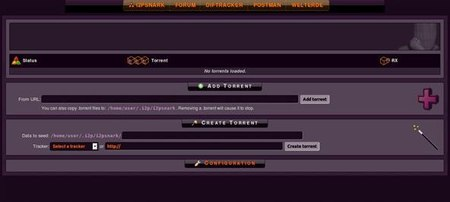
\includegraphics[width=1\textwidth]{media/i2p_3.jpg}
    \caption{Captura de I2PSnark.}
    \label{fig5}
\end{figure}


\subsection{PyBitmessage[6]}
Es un servicio de correo electrónico que permite recibir o enviar bitmessages a traves de I2P,funciona cifrando todos los mensajes de entrada y salida
usando criptografía asimétrica de modo que solo receptor es capaz de poder descifrar el mensaje del emisor.
\\

Destacamos que permite enviar correo a traves de internet,Tor e I2P y ofrece webmail,pop3,IMAP y SMTP,su funcionamiento es muy parecido a un cliente de correos
pero con las ventajas de que la comunicación entre  emisor y receptor es confidencial, está asegurada la confidencialidad de dicha comunicación.  
\\

Para usar PyBitMessage  primero instalamos las siguientes dependencias : python2.7,python2-qt4 (python-qt4 en ubuntu),openssl.(si usamos  Fedora y Redhat añadir openssl-compat-bitcoin-libs).
\\

Tras instalar las dependencias podemos ejecutar PyBitmessage de dos formas,descargamos PyBitmessage y ejecutamos directamente python desde el código fuente o a través de un paquete 
instalable en en el sistema. Dado que PyBitmessage es Beta, es mejor  ejecutar PyBitmessage desde el código fuente, para que pueda actualizarse si fuese necesario.
\\

\begin{figure}[H]
    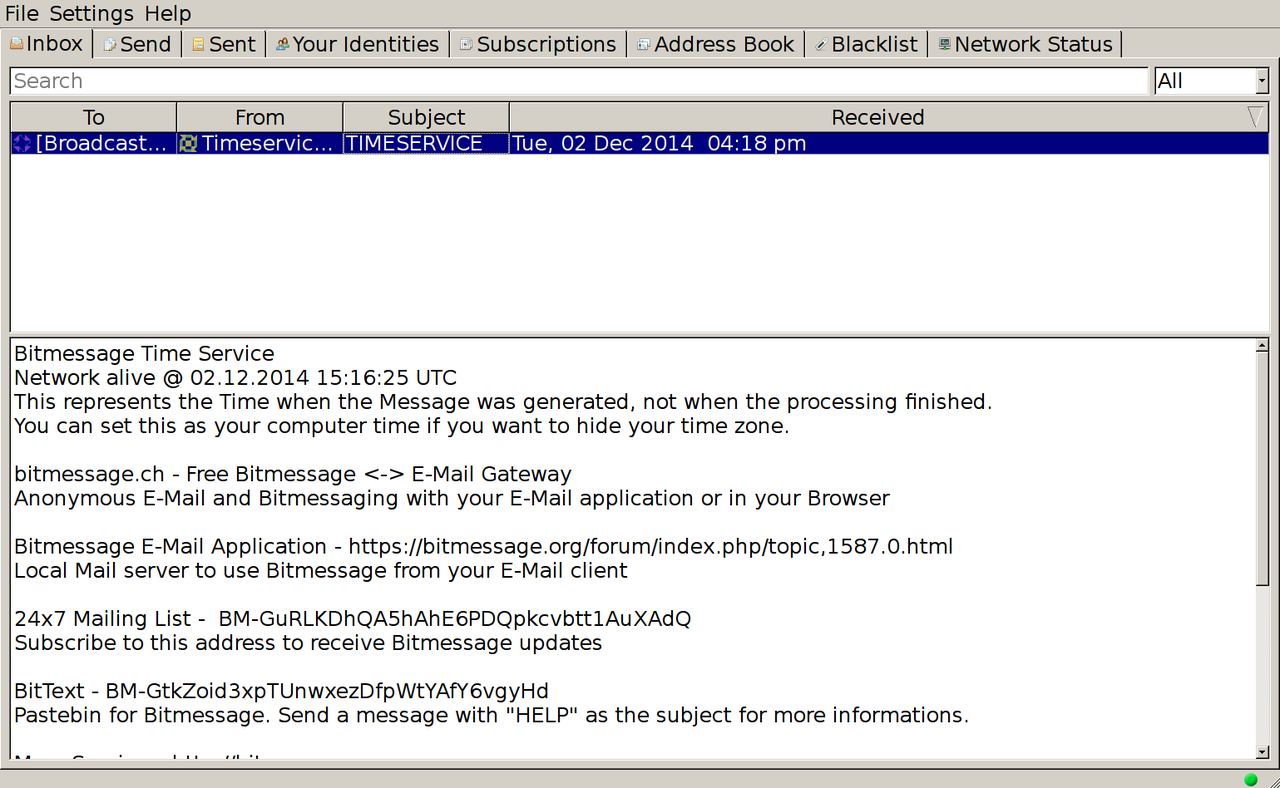
\includegraphics[width=1\textwidth]{media/PyBitMessage-client.png}
    \caption{Captura de pyBitmessage.}
    \label{fig6}
\end{figure}

Estos son unos  ejemplos de los muchos software que existen , que usan I2P ,pero actualmente existen muchos software que esta en continuo desarrollo debido a que 
I2P sigue creciendo debido a el interés de preservar nuestro anonimato.

\pagebreak

\section{Conclusión}
Hoy dia, nuestros datos e identidad son muy importantes,navegar sin que estos esten protegidos o cifrados contribuye a que cada dia estemos expuesto
a el robo de  nuestra información más personal y más importante aun,alguien con conocimiento podría identificarnos ya que nuestro anonimato no esta asegurado 
poniendo en riesgo lo más importante nuestra identidad unica, Sin embargo haciendo uso de tecnologia como I2P ,la cual  están en continuo desarrollo,
permiten nuestro anonimato, protegiendo así nuestra identidad y nuestra actividad en las redes, la cual es continuamente rastreada.

\pagebreak

\section{Referencias}

[1] https://www.genbeta.com/actualidad/i2p-la-nueva-generacion-de-la-deep-web 
[2] http://scielo.sld.cu/scielo.php?script=sci\_arttext\&pid=S2218-36202017000200014
[3] http://repositorio.ug.edu.ec/bitstream/redug/17047/1/UG-FCMF-B-CINT-PTG-N.106.pdf
[4] https://geti2p.net/es/docs/api/i2ptunnel 
[5] https://www.ghacks.net/2007/06/06/anonymous-bittorrent-with-i2psnark/ 
[6] https://es.wikipedia.org/wiki/Bitmessage\#Bitmessage.ch 
[7] https://dl.acm.org/doi/10.1145/358549.358563 
[8] https://geti2p.net/en/download 
[9] https://geti2p.net/en/faq\#systems 
[10] https://arstechnica.com/information-technology/2015/01/under-the-hood-of-i2p-the-tor-alternative-that-reloaded-silk-road/ 
[11] https://i2pd.readthedocs.io/en/latest/user-guide/tunnels/ 



\section{Funcionamiento}
\section{Utilidades}
\section{Diferencia respecto a otras tecnologías}
\subsection{Ventajas}
\subsection{Inconvenientes}
\section{I2P sobre linux}
\section{Bibliografía}
\begin{itemize}
    \item %http://scielo.sld.cu/scielo.php?script=sci\_arttext&pid=S2218-36202017000200014
\end{itemize}
\end{document}
